
\section{Newton's Laws and Momentum Conservation\footnote{
1990-93 Dept. of Physics and Astronomy, Dickinson College. Supported by FIPSE
(U.S. Dept. of Ed.) and NSF. Portions of this material may have been modified
locally and may not have been classroom tested at Dickinson College.
}}

\makelabheader %(Space for student name, etc., defined in master.tex or labmanual_formatting_commands.tex)

\textbf{Objectives }

\begin{itemize}
\item To study the forces between objects that undergo collisions and other types
of interactions in a short time period. 
\item To formulate the Law of Conservation of Momentum as a theoretical consequence
of Newton's laws and to test it experimentally.
\end{itemize}
\textbf{Apparatus}

\begin{itemize}
\item 2 force probes (force sensors)
\item Rubber bumpers, hooks and springs for the force probes
\item 2 Pasco dynamics carts
\item A track for the dynamics carts
\item A video analysis system (\textit{Tracker})
\item A movie scaling ruler
\item Graphing and curve fitting software (\textit{Excel})
\item Circular bubble level
\item Pasco 550 Interface
\item \textit{Capstone} software (\filename{Two\_Force\_Probes.cap} experiment file)
\end{itemize}
\textbf{Predicting Interaction Forces between Objects} 

We recently focused our attention on the change in momentum that an object undergoes
when it experiences a force that is extended over time (even if that time is
very short!). Since interactions like collisions and explosions never involve
just one object, we would like to turn our attention to the mutual forces of
interaction between two or more objects. As usual, you will be asked to make
some predictions about interaction forces and then be given the opportunity
to test these predictions. 

\textbf{Activity 1: Predicting Interaction Forces} 

(a) Suppose the masses of two objects are the same and that the objects are
moving toward each other at the same speed so that
\[
m_{1}=m_{2}\quad \mbox{and}\quad {{\bf v}_{1}}=-{{\bf v}_{2}}\]


\vspace{0.3cm}
{\par\centering 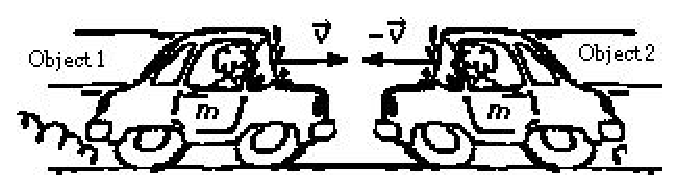
\includegraphics{newtons_laws/newtons_laws_fig1.eps} \par}
\vspace{0.3cm}

\pagebreak[2]

Predict the relative magnitudes of the forces between object 1 and object 2.
Place a check next to your prediction! 

\rule{0.5in}{0.1pt} Object 1 exerts more force on object 2. 

\rule{0.5in}{0.1pt} The objects exert the same force on each other. 

\rule{0.5in}{0.1pt} Object 2 exerts more force on object 1.

(b) Suppose the masses of two objects are the same and that object 1 is moving
toward object 2, but object 2 is at rest.
\[
m_{1}=m_{2}\quad \mbox{and}\quad {{\bf v}_{1}}>{{\bf v}_{2}}\]


\vspace{0.3cm}
{\par\centering 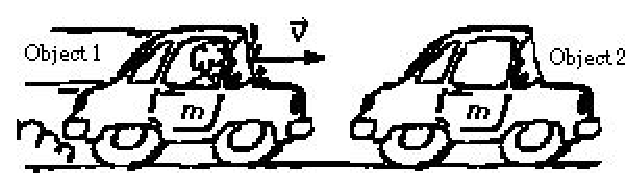
\includegraphics{newtons_laws/newtons_laws_fig2.eps} \par}
\vspace{0.3cm}

Predict the relative magnitudes of the forces between object 1 and object 2.
Place a check next to your prediction! 

\rule{0.5in}{0.1pt} Object 1 exerts more force on object 2. 

\rule{0.5in}{0.1pt} The objects exert the same force on each other.

\rule{0.5in}{0.1pt} Object 2 exerts more force on object 1.

(c) Suppose the mass of object 1 is much less than that of object 2 and that
it is pushing object 2 that has a dead motor so that both objects move in the
same direction at speed v.
\[
m_{1}\ll m_{2}\quad \mbox{and}\quad {{\bf v}_{1}}={{\bf v}_{2}}\]


\vspace{0.3cm}
{\par\centering 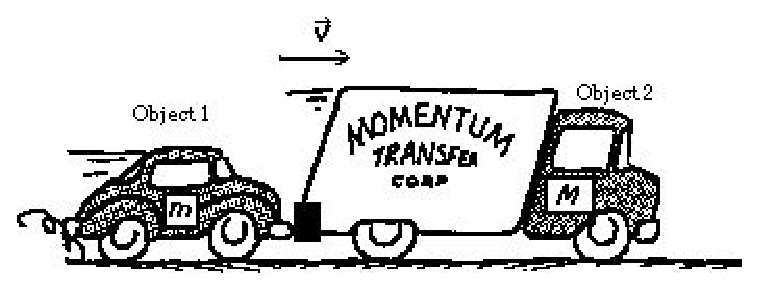
\includegraphics{newtons_laws/newtons_laws_fig3.eps} \par}
\vspace{0.3cm}

Predict the relative magnitudes of the forces between object 1 and object 2.
Place a check next to your prediction. 

\rule{0.5in}{0.1pt} Object 1 exerts more force on object 2. 

\rule{0.5in}{0.1pt} The objects exert the same force on each other. 

\rule{0.5in}{0.1pt} Object 2 exerts more force on object 1.

(d) Suppose the mass of object 1 is greater than that of object 2 and that the
objects are moving toward each other at the same speed so that
\[
m_{1}>m_{2}\quad \mbox{and}\quad {{\bf v}_{1}}=-{{\bf v}_{2}}\]


%\vspace{0.3cm}
{\par\centering 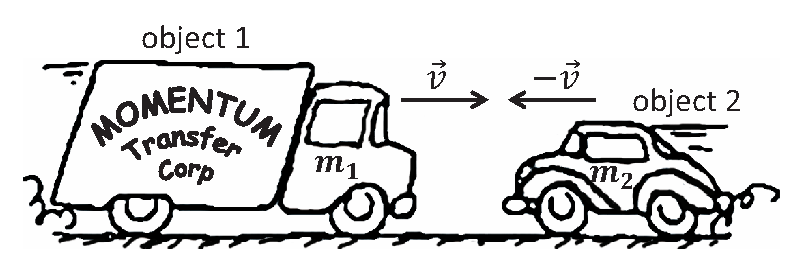
\includegraphics{newtons_laws/newtons_laws_fig4_new.eps} \par}
%\vspace{0.3cm}

Predict the relative magnitudes of the forces between object 1 and object 2.
Place a check next to your prediction. 

\rule{0.5in}{0.1pt} Object 1 exerts more force on object 2. 

\rule{0.5in}{0.1pt} The objects exert the same force on each other.

\rule{0.5in}{0.1pt} Object 2 exerts more force on object 1.

(e) Suppose the mass of object 1 is greater than that of object 2 and that object
2 is moving in the same direction as object 1 but not quite as fast so that
\[
m_{1}>m_{2}\quad \mbox{and}\quad {{\bf v}_{1}}>{{\bf v}_{2}}\]


\vspace{0.3cm}
{\par\centering 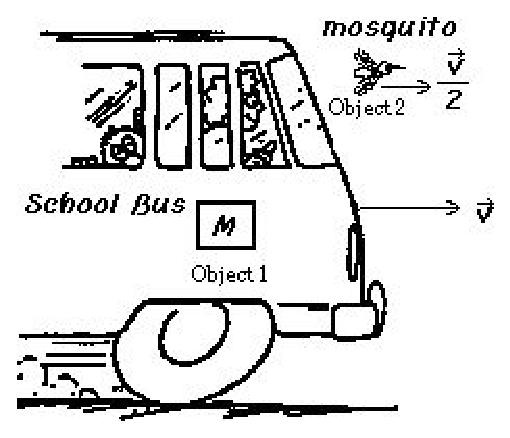
\includegraphics{newtons_laws/newtons_laws_fig5.eps} \par}
\vspace{0.3cm}

Predict the relative magnitudes of the forces between object 1 and object 2.
Place a check next to your prediction. 

\rule{0.5in}{0.1pt} Object 1 exerts more force on object 2. 

\rule{0.5in}{0.1pt} The objects exert the same force on each other. 

\rule{0.5in}{0.1pt} Object 2 exerts more force on object 1.

(f) Suppose the mass of object 1 is greater than that of object 2 and that both
objects are at rest until an explosion occurs, so that
\[
m_{1}>m_{2}\quad \mbox{and}\quad {{\bf v}_{1}}={{\bf v}_{2}}=0\]


\vspace{0.3cm}
{\par\centering 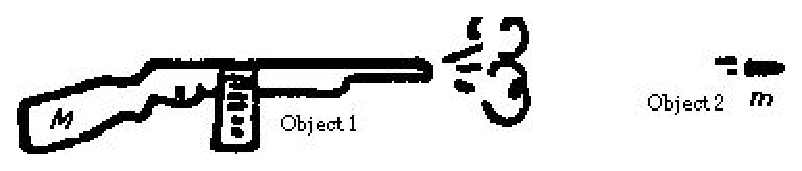
\includegraphics{newtons_laws/newtons_laws_fig6.eps} \par}
\vspace{0.3cm}

Predict the relative magnitudes of the forces between object 1 and object 2.
Place a check next to your prediction. 

\rule{0.5in}{0.1pt} Object 1 exerts more force on object 2. 

\rule{0.5in}{0.1pt} The objects exert the same force on each other. 

\rule{0.5in}{0.1pt} Object 2 exerts more force on object 1.

(g) Provide a summary of your predictions. What are the circumstances under
which you predict that one object will exert more force on another object?
\answerspace{30mm}

\textbf{Measuring Mutual Forces of Interaction }

In order to test the predictions you made in the last activity you can study
gentle collisions between two force probes attached to carts. First, open the file \filename{Two\_Force\_Probes.cap}
in the \filename{\coursefolder} folder.  Calibrate both force probes 
(see \textit{Calibrating Force Sensors} in \textbf{Appendix \ref{capstone}: Capstone}). 
For this experiment, set the 2nd calibration point to 1.96~N for one force probe and $-1.96$~N for the other, so that they read forces with opposite signs. 
You can strap additional masses to one of the carts to increase its total mass so it has significantly
more mass than the other. If a compression spring is available you can set up
an ``explosion'' between the two carts by compressing the spring
between the force probes on each cart and letting it go. You can make and display the force measurements with the Two Force Probes file already opened. You can also determine the areas under the force \textit{vs.}~time graphs to find the impulses experienced by the carts during the collisions. See \textbf{Appendix \ref{capstone}: Capstone} for instructions on finding the area under a curve.

\textbf{Activity 2: Measuring Slow Forces} 

(a) Play a gentle tug-of-war in which you pull the ends of the two force probes away from each other for about 10 seconds with your partner using the hooks on the force probes hooked together. What do you observe about the mutual forces?
\answerspace{20mm}

(b) Remove the hooks and attach rubber bumpers to the two force probes. Play a gentle tug-of-war in which you push the ends of two force probes against each other for about 10 seconds with your partner. What do you observe about the mutual forces?
\answerspace{20mm}

(c) Now that you're warmed up to this two force measurement technique go ahead and
try some different types of gentle collisions between two carts of different
masses and initial velocities. To do this, remove the rubber bumpers and attach springs to the two force probes.

\pagebreak[3]
\textbf{Activity 3: Measuring Collision Forces }

(a) Use the two carts to explore various situations that correspond to the predictions
you made about mutual forces. Your goal is to find out under what circumstances
one object exerts more force on another object. Describe what you did in the
space below and attach a printout of at least one of your graphs of force 1 \textit{vs.}~time and force 2 \textit{vs.}~time.
\answerspace{30mm}

(b) What can you conclude about forces of interactions during collisions? Are there any circumstances under which one object experiences a different magnitude of force
than another during a collision? How do the magnitudes and directions of the
forces compare on a moment by moment basis in each case? 
Compare your answers here with your predictions.
\answerspace{30mm}

(c) Do your conclusions have anything to do with Newton's third law?
\answerspace{20mm}

(d) How does the vector impulse due to object 1 acting on object 2 compare to
the impulse of object 2 acting on object 1 in each case? Are they the same in
magnitude or different? Do they have the same sign or a different sign? Remember
\( {\bf I}=\int _{t_{i}}^{t_{f}}{\bf F}\,dt \).
\vspace{20mm}

\textbf{Newton's Laws and Momentum Conservation} 

In your investigations of interaction forces, you should have found that the
forces between two objects are equal in magnitude and opposite in sign on a
moment by moment basis for all the interactions you studied. This is of course
a testimonial to the seemingly universal applicability of Newton's third law
to interactions between ordinary masses. You can combine the findings of the
impulse-momentum theorem (which is really another form of Newton's second law
since we derived it mathematically from the second law) to derive the Law of
Conservation of Momentum shown below.

{\par\centering \textbf{Law of Conservation of Momentum}
\[
\sum {\bf p}={{\bf p}_{1i}}+{{\bf p}_{2i}}={{\bf p}_{1f}}+{{\bf p}_{2f}}=
\mbox{constant in time}\]
\par}

where 1 refers to object 1 and 2 refers to object 2 and $i$ refers to the initial
momenta and $f$ to the final momenta.

\pagebreak[2]

\textbf{Activity 4: Deriving Momentum Conservation }

(a) What did you conclude in the last activity about the magnitude and sign
of the impulse on object 1 due to object 2 and vice verse when two objects interact?
In other words, how does \( {{\bf I}_{1}} \) compare to \( {{\bf I}_{2}} \)? 
\vspace{10mm}

(b) Since you have already verified experimentally that the impulse-momentum
theorem holds, what can you conclude about how the change in momentum of object
1, \( \Delta {{\bf p}_{1}} \), as a result of the interaction compares
to the change in momentum of object 2, \( \Delta {{\bf p}_{2}} \),
as a result of the interaction? Remember \( {\bf I}=\Delta {\bf p} \).
\vspace{25mm}

(c) Use the result of part (b) to show that the Law of Conservation
of Momentum holds for a collision, i.e. \( \sum {\bf p} 
=  {{\bf p}_{1i}}  + {{\bf p}_{2i}}  = {{\bf p}_{1f}} 
+ {{\bf p}_{2f}} \) = constant in time.
\vspace{20mm}

In the next few units you will continue to study one- and two-dimensional collisions
using momentum conservation. Right now you will attempt to test the Law of Conservation
of Momentum for a simple situation by using video analysis. To do this you will
make and analyze a video movie in which two carts of DIFFERENT masses undergo
a one-dimensional elastic collision. You may not be able to finish this in class,
but you can complete the project for homework.

\textbf{Testing Momentum Conservation }

You just used theoretical grounds to derive momentum conservation. This idea
still must be tested against experiment. You will make this test by colliding
two carts (of different masses) on a track and recording and analyzing their motion 
before and after they hit. Measure the masses of the carts and record the total mass 
of each cart here:

\vspace{10mm}

\textbf{Activity 5: Colliding Carts }

(a) Make a movie of two carts colliding by following these steps. 

\begin{enumerate}
\item Open \textbf{Camera} and turn on the camera as explained in \textbf{Appendix \ref{tracker}: Video Analysis Using Tracker}. Center the track in the field of view of the 
camera which should be about 1 m above the center of the track where one cart (the target) will
sit. The target cart should be located straight down below the camera. Align the track so that it is parallel to the border of the movie image. Make sure the track is level by using the small level available at each station. Place a ruler somewhere in the field of view where it won't interfere with the collision. This ruler will be used later to determine the scale. 
\item Make a movie of one cart (the projectile) rolling into the other, stationary
cart (the target). See \textbf{Appendix \ref{tracker}: Video Analysis Using Tracker} for details on making the movie. When you save the movie file give it the name \textit{Collision}.
\end{enumerate}
(b) Determine the position of both carts (the target and the projectile) during
the motion using \textit{Tracker}. In \textit{Tracker}, align one of the axes along the path 
of the incoming projectile. Track one cart, then the other as functions of time. For each cart 
you will have a table showing values of time and x position for each cart.
% If using \textbf{VideoPoint}, follow the instructions in \textbf{Appendix \ref{videopoint}: Video
%Analysis} for recording and calibrating the video data. NOTE: Under 
%\textbf{Analyzing the Movie} in \textbf{Appendix \ref{videopoint}}, number 2 says 
%$VideoPoint$ will request the number of objects you want to track. BE SURE TO 
%ENTER 2 FOR THIS NUMBER so that you can mark two objects on
%each frame; click once on the projectile cart and once on the target cart. The
%data table should contain five columns with the values of time, x and y 
%positions of the projectile cart, and x and y positions of the target cart. 
%Note: Since this is a horizontal 1D collision the y-coordinates are of no 
%interest. They should be constant for each frame. If they are not, consult 
%your instructor.

(c) Within \textit{Tracker}, create graphs of position versus time for both carts. Print the 
graphs and include them with this unit. You can determine the initial and final velocities 
of each cart from the slopes of the appropriate segments of the graphs.

(d) Use your data to calculate the momenta of carts 1 and 2 before the collision.
\vspace{25mm}

(e) Use the data to calculate the momenta of carts 1 and 2 after the collision.
\vspace{25mm}

(f) Using the results of parts (d) and (e), calculate the total momentum before and after the collision. 
Also calculate the difference between the total momentum before and after the collision ($p_f - p_i$) and 
the percent difference $(p_f - p_i)/p_{ave}$ (where $p_{ave}$ is the average of $p_i$ and $p_f$), and record them below.
Go around to the other lab groups and get their results for the difference $p_f - p_i$.
Make a histogram of the results you collect and calculate the average and standard deviation.
For information on making histograms, see \textbf{Appendix \ref{excel}}. 
For information on calculating the average and standard deviation, see \textbf{Appendix \ref{treatment}}. Record the average and standard 
deviation here. Attach the histogram to this unit.
\vspace{35mm}

(g) What is your expectation for the difference between the initial and final momentum? 
Do the data from the class support this expectation?  
Use the average and standard deviation for the class to quantitatively answer this question.
\vspace{20mm}

(h) What does the histogram of the class data tell you?
\vspace{20mm}

(i) Within the limits of experimental uncertainty, is momentum 
conserved (i.e., is the total momentum of the two cart system the same before
and after the collision)?

